% Made up for the tikra benchmark.
% The tower of Hanoi with five disks, in the middle of being solved.
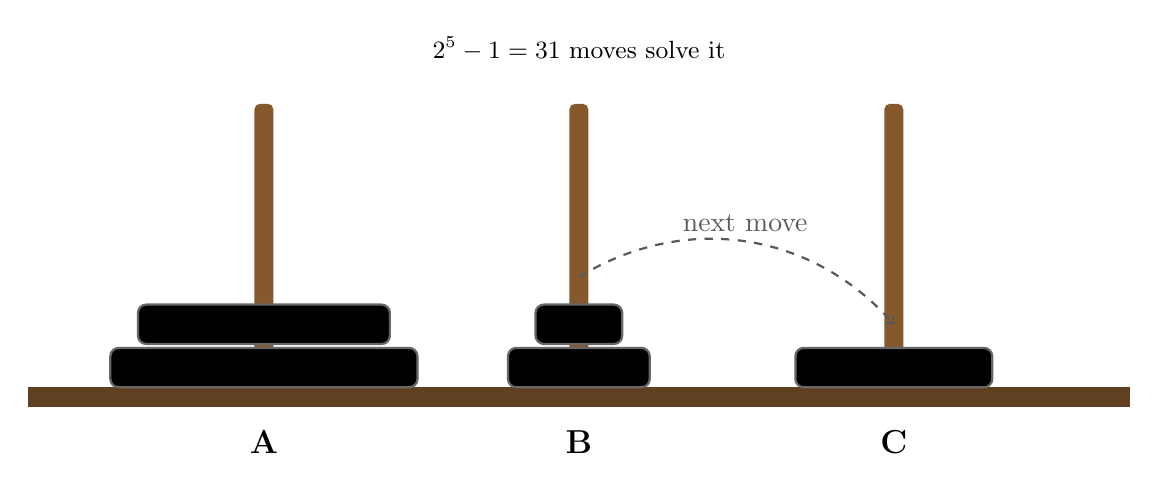
\begin{tikzpicture}[disk/.style={rounded corners=3pt, draw=black!60, thick}]
  \fill[brown!50!black] (-1,-0.25) rectangle (13,0);
  \foreach \x/\name in {2/A, 6/B, 10/C} {
    \fill[brown!70!black, rounded corners=2pt] (\x-0.12,0) rectangle (\x+0.12,3.6);
    \node[font=\large\bfseries] at (\x,-0.7) {\name};
  }
  \foreach \peg/\level/\size/\color in {2/0/5/red!70, 2/1/4/orange!80, 10/0/3/yellow!80!orange, 6/0/2/green!60, 6/1/1/blue!50} {
    \fill[\color, disk] (\peg-0.35*\size-0.2, \level*0.55) rectangle (\peg+0.35*\size+0.2, \level*0.55+0.5);
  }
  \draw[->, thick, dashed, gray!70!black] (6,1.4) to[bend left=40] node[above] {next move} (10,0.8);
  \node[font=\small] at (6,4.3) {$2^5 - 1 = 31$ moves solve it};
\end{tikzpicture}
